\documentclass[../main/main.tex]{subfiles}

\newdate{date}{6}{12}{2019}


\begin{document}

\marginpar{ \textbf{Lecture 16.} \\  \displaydate{date}. \\ Compiled:  \today.}

\section{Cubic term and first transition}
Let us consider more general forms of the Landay free energy. For example, in the case in which the symmetry is not violated, one can consider also odd temrs such as the cubic one.  In fact, we want to eneralize to include multicritical points, or phase transitions. The phase transitions can be obtained by introducing a cubic term in the Landau expansion. Remember that in the Ising model we have phase transition derived by symmetry breaking. Now, we have another type of phase transition.

The simplest Landau free energy that depends on a particular field is:
\begin{equation}
  \mathcal{L} ( \eta ,t,h)= a t \eta ^2 - w \eta ^3 + \frac{b}{4} \eta ^4 - h \eta
\end{equation}
where \( t \equiv \frac{T-T^*}{2} \) and \( w \) is an additional parameter that we fix to be positive, \( w>0 \).
\begin{remark}
For \( w<0 \) the results are the same, but in the \( \eta <0 \) diagram.
\end{remark}
To satisfy thermodynamic stability we require \( b>0 \), while
\begin{equation}
  a t = \frac{a}{2} ( T - T^*) \quad \text{if } \begin{cases}
    > 0 & T > T^* \\
    <0 & T < T^*
\end{cases}
\end{equation}
The equation of state for \( h \neq 0 \) is:
\begin{equation}
  \pdv{\mathcal{L}_G}{\eta } = 0 \quad \Rightarrow h = 2 a t \eta - 3 w \eta ^2 + b \eta ^3
\end{equation}
Let us consider the equilibrium states when \( h=0 \):
\begin{equation}
  h = 0 \quad \Rightarrow 0 = \eta ( 2 a t - 3 w \eta  + \beta \eta ^2)
\end{equation}
 The possible solutions are
\begin{equation}
  \begin{cases}
   \bar{\eta } = 0 & \text{disordered phase}\\
  \bar{\eta } = \frac{1}{4b} \qty(3w \pm \sqrt{q w^2 - 16 abt} ) & \text{ordered phases}
  \end{cases}
\end{equation}
Let us rewrite the 'ordered' solutions as
\begin{equation}
  \bar{\eta }_{\pm} = c \pm \sqrt{c^2 - \frac{at}{b}}
\end{equation}
where
\begin{equation}
  c = \frac{3w}{4b}
\end{equation}
Note that
\begin{equation}
  \bar{\eta }_{\pm} \in \R \iff c^2 > \frac{at}{b} \quad \Rightarrow \frac{T-T^*}{2} < \frac{c^2 b}{a} \equiv t^{**} \equiv  \frac{T^{**}-T^*}{2}
\end{equation}
It implies:
\begin{equation}
  T^{**} = T^* + \frac{2c^2b}{a}
\end{equation}
\begin{itemize}
\item If \( t> t^{**} \) \( (\iff T > T^ {**}) \), we have  \( \bar{\eta }_\pm \notin \R  \). The only real solution is \( \bar{\eta }=0  \) that is also the absolute minimum of \( \mathcal{L} \). The plot is shown in Figure \ref{fig:16_1}.
\begin{figure}[h!]
\centering
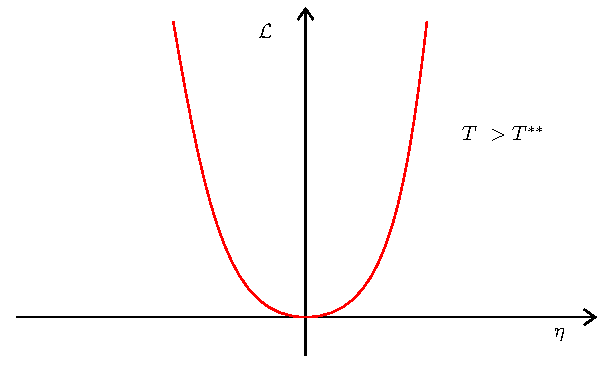
\includegraphics[width=0.6\textwidth]{../lessons/16_image/1.pdf}
\caption{\label{fig:16_1} Description.}
\end{figure}

\item If \( t \le t^{**} \) \( (\iff T \le T^ {**}) \), we have \( \bar{\eta }_\pm = c \pm \sqrt{c^2 - \frac{at}{b}} \in \R  \) are both possible solutions. One will be a local maximum and the other a local minimum.

\begin{itemize}
\item At \( T = T^{**}\), \( \bar{\eta }_- = \bar{\eta }_+   \) (flex point), as shown in Figure \ref{fig:16_2}.
\begin{figure}[h!]
\centering
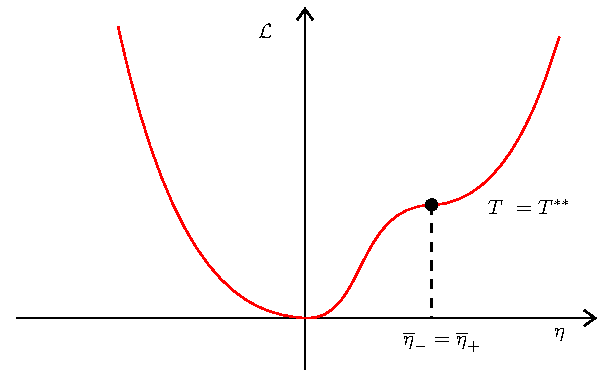
\includegraphics[width=0.6\textwidth]{../lessons/16_image/2.pdf}
\caption{\label{fig:16_2} Description.}
\end{figure}
\item For \( T_t < T < T^{**} \), \( \mathcal{L} (\bar{\eta }_+) >0  \). Since \( \mathcal{L} (\bar{\eta }=0 ) \), the solution \( \bar{\eta }_+  \) is a local minimum, as shown in Figure \ref{fig:16_3}.
\begin{figure}[h!]
\centering
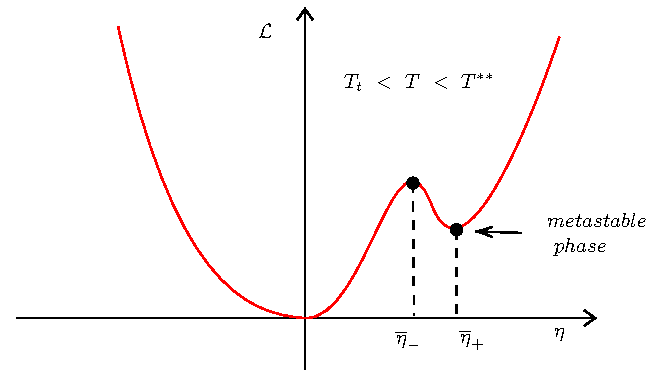
\includegraphics[width=0.6\textwidth]{../lessons/16_image/3.pdf}
\caption{\label{fig:16_3} Description.}
\end{figure}
\item By decreasing \( T \) firther one eventually reaches the value \( T=T_t \) at which the local minimum \( \mathcal{L} (\bar{\eta }_+ ) \) becomes zero, as in Figure \ref{fig:16_4}. \( T_t \)  is given by the coexistence condition
\begin{equation}
  \mathcal{L} (\bar{\eta }_+ ) = \mathcal{L} (0)
\end{equation}
that is the coexistence between the disordered and ordered phases!
\begin{figure}[h!]
\centering
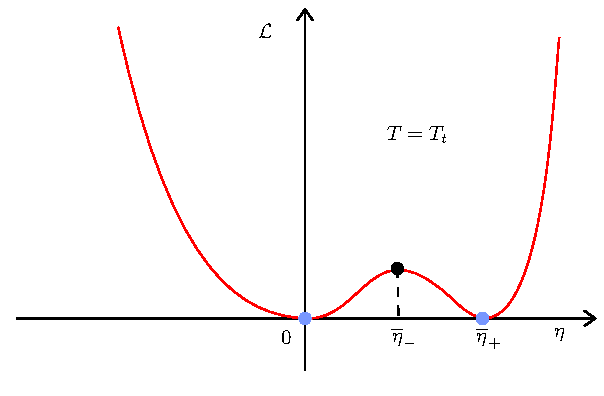
\includegraphics[width=0.6\textwidth]{../lessons/16_image/4.pdf}
\caption{\label{fig:16_4} Description.}
\end{figure}

In the plot of Figure \ref{fig:16_4} we see that there are two minima in the same line, this is  a first order transition.
At \( T=T_t \) the system undergoes a first order transition. To determine \( T_t \) we consider
\begin{equation}
  \begin{cases}
   \pdv{\mathcal{L}}{\eta } = 0 = \eta \qty(2 a t - 3 w \eta + 2 b \eta ^2)  & \text{extreme condition}\\
  \mathcal{L} ( 0 ) = \mathcal{L} ( \eta _+) & \text{coexistence condition}
  \end{cases}
\end{equation}
\begin{equation}
\Rightarrow
  \begin{cases}
   2 a t - 3 w \eta + 2 b \eta ^2 = 0\\
   a t - w \eta + \frac{b}{2} \eta ^2 = 0
  \end{cases}
\end{equation}
Solving with respect to \( \eta  \)  and \( t \) we get
\begin{equation}
  \begin{cases}
   \bar{\eta }_{+t} = + \frac{w}{b} >0 \\
    t_t = \frac{w^2}{2ba} \equiv \frac{1}{2} (T_t - T^*)
  \end{cases}
\end{equation}
\begin{equation}
  T_t = \frac{w^2}{b a} + T^*
\end{equation}
\begin{remark}
Note that \( T_t >T^* \).
\end{remark}
Since at \( T= T_t \) there is a first order transition does the system display latent heat?
\begin{equation}
  s = \eval{- \pdv{\mathcal{L}}{T} }_{\eta _t} = - \frac{1}{2} a \bar{\eta }_t^2 = - \frac{a}{2} \qty(\frac{w}{b})^2
\end{equation}
\begin{remark}
There is an entropy jump.
\end{remark}
The latent heat adsorbed to go from the ordered to the disordred phase is
\begin{equation}
  q = - T_t s = \frac{a}{2} T_t \qty(\frac{w}{b})^2
\end{equation}

\item Finally for \( T^* < T < T_t \), \( \eta = \bar{\eta }_+  \) becomes the global minimum ordered phase is the only stable one (Figure \ref{fig:16_5}).
\begin{figure}[h!]
\centering
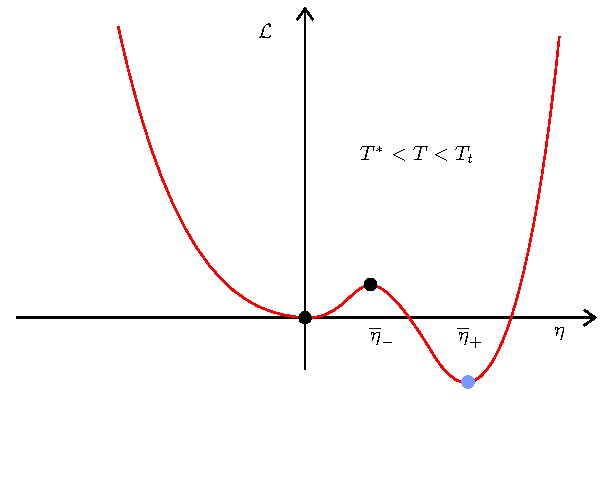
\includegraphics[width=0.6\textwidth]{../lessons/16_image/5.pdf}
\caption{\label{fig:16_5} Description.}
\end{figure}
\end{itemize}
\end{itemize}


\section{Phase stability and behaviour of \( \chi _T \equiv \pdv{\eta }{h}  \)}

Let us derive the equation of state with respect to \( h \)
\begin{equation}
  \pdv{}{h} \qty(\pdv{\mathcal{L}_G}{\eta } = 0 )   = \pdv{}{h} \qty(2 a t \eta - 3 w \eta ^2 + 2 b \eta ^3 = h)
\end{equation}
\begin{equation}
  \Rightarrow \chi \qty(2 a t - 6 w \eta + 6 b \eta ^2 ) =1
\end{equation}
The results is
\begin{equation}
  \chi _T = \frac{1}{2 a t - 6 w \eta + 6 b \eta ^2}
  \label{eq:16_1}
\end{equation}
We now make use of equation \eqref{eq:16_1} to compute the limit of stability of the phases we have found.

\subsection{Computation of \( T^{**} \) }
\( T=T^{**} \) is the value below which the ordred phase \( (\bar{\eta } = \bar{\eta }_+ ) \) becomes a metastable state (local minima). Since this coincides with the flex point
\begin{equation}
  \pdv[2]{\mathcal{L}}{\eta } = 0 \quad \Rightarrow \chi ^{-1} = 2 a t - 6 w \eta + 6 b \eta ^2 = 0
\end{equation}
Remember that at \( T=T{**} \)  the two solutions \( \eta _\pm \) do coincide
\begin{equation}
  c^2 - \frac{at}{b} = 0 \Rightarrow \eta _\pm = \eta _2 = \frac{3 w}{4 b}
\end{equation}
Inserting in the expression for \( \chi ^{-1} \) since \( \chi ^{-1} =0 \) we have
\begin{equation}
  \chi ^{-1} = 0 = 2 a t^{**} - 6 w \bar{\eta }_2 + 6 \bar{\eta }_2^2
\end{equation}
\begin{equation}
  \iff t^{**} = \frac{q w^2}{16 a b} = \frac{1}{2} \qty(T^{**}-T^*)
\end{equation}
For \( T_t < T < T^{**} \) the ordered phase is metastable.

\subsection{Computation of \( T^* \)}
The instability of the disordered phase \( (\eta =0) \) is when \( \mathcal{L} \) presents a flex point at \( \eta =0 \), as in Figure \ref{fig:16_6}.
\begin{equation}
  \chi ^{-1} (\eta =0) = 0 \iff \chi ^{-1} (\eta =0) = 2 a t = 0 \iff t = 0 \quad \Rightarrow T = T^*
\end{equation}

\begin{figure}[h!]
\centering
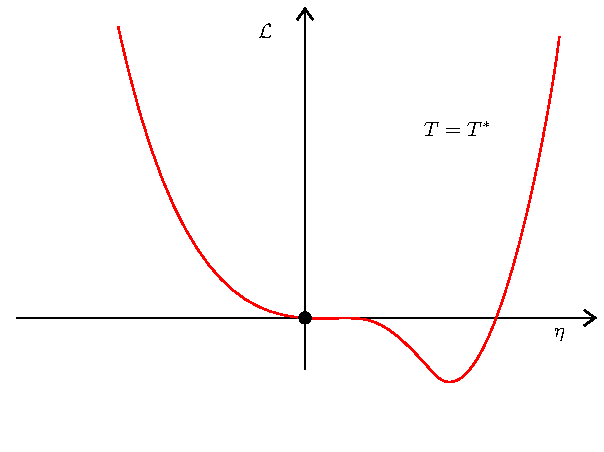
\includegraphics[width=0.6\textwidth]{../lessons/16_image/6.pdf}
\caption{\label{fig:16_6} Description.}
\end{figure}


\section{Landau theory and multicritical points}
Tricritical point is a critical point that separates a line of first transition points from a line of critical points.
\begin{remark}
The introduction of a cubic term is not the only way to obtain a first order transition. Let allow the coefficient of \( \eta ^4 \) to change signs. We need the \( \eta ^6 \) term (See Blume-Emery-Griffith model).
\end{remark}
\begin{equation}
  \mathcal{L}_h (T, \Delta, \eta ) = \frac{a (t,\Delta )}{2} \eta ^2 + \frac{b(t,\Delta )}{4} \eta ^4 + \frac{c}{6} \eta ^6 - h \eta
\end{equation}
where we have two parameteres \( (T,\Delta ) \) and \( c>0 \), with \( \Delta  \) that is the disordered field (\( \% \, \text{He}^3\) in the BEG model).

Now, consider \( \Delta  \) (\( \Delta _c \) is a critical value). The phenomenology is

\begin{itemize}
\item \( \Delta < \Delta _c \): as \( T \) decreases, \( a(T,\Delta ) \) decreases and at \( T = T_c (\Delta ) \) becomes zero. In this region \( b(T,\Delta ) >0 \) and the system displays the standard \( (\eta ^4) \) critical point.
\begin{equation}
  T = T_c (\Delta ) \Rightarrow \begin{cases}
    a (T_c,\Delta ) = 0 \\
    b (T_c,\Delta ) > 0
\end{cases}
\end{equation}
\item \( \Delta > \Delta _c \): as \( T \) decreases, \( b(T,\Delta ) \) becomes zero 'before' \( a(T,\Delta ) \). In this case one can show the existence of a line of first transition points:
\begin{equation}
  b (\bar{T},\Delta  ) = 0 \quad \Rightarrow   \mathcal{L} = a \eta ^2 + c \eta ^6, \quad a>0
\end{equation}
\begin{equation}
  \pdv{\mathcal{L}}{\eta } = 2 a \eta + 6 c \eta ^5 \Rightarrow \begin{cases}
    \eta =0 \\
    \eta _{1,2,3,4}
  \end{cases}
\end{equation}

\begin{figure}[h!]
\centering
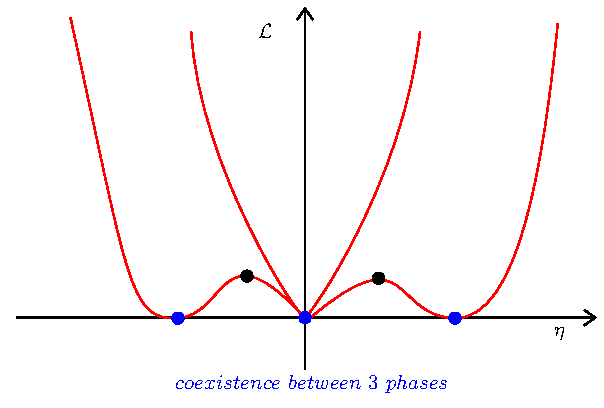
\includegraphics[width=0.6\textwidth]{../lessons/16_image/7.pdf}
\caption{\label{fig:16_7} Description.}
\end{figure}

If \( b>0 \), \( \eta ^6 \) can be neglected.
\item The Tricritical point is given by the values of \( \Delta = \Delta _t \)  and \( T= T_c \) such that
\begin{equation}
  a (\Delta _t, T_t) = b (\Delta _t, T_t) = 0
\end{equation}
At this point the system is described by the following Landau free-energy
\begin{equation}
  \mathcal{L}_t = c \eta ^6 - h \eta
\end{equation}
and equation of state
\begin{equation}
  h = 6 c \eta ^5
\end{equation}

\begin{figure}[h!]
\centering
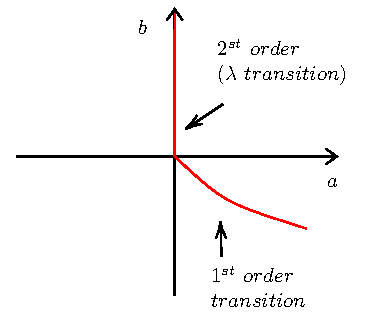
\includegraphics[width=0.6\textwidth]{../lessons/16_image/8.pdf}
\caption{\label{fig:16_8} Description.}
\end{figure}

\end{itemize}

\section{Landau-de Gennes theory of liquid crystals}
A liquid crystal phase (LC) can be seen as an intermediate phase (mesophase) between a solid and a liquid phase.
In this phase the system flows as a fluid but it also displays an orientational order typical of a crystal. Because of this order this phase displays \emph{anisotropic} optical, magnetic and electrical properties.

Typical structural properties of the elementary constituents (molecules) giving rise to LC phase are the following
\begin{itemize}
\item Anisotropic (elangated) shape.
\item The long axis can be approximated as a rigid backbane.
\item Existence of strong dipoles and groups easy to polarize.
\end{itemize}
\subsection{LC-phases}
There are many possible LC phase, from \emph{nematic}, \emph{cholesteric}, \emph{smectic}, \emph{columnar}, etc. Here we gocus on the most common one the \emph{nematic phase}.

The nematic phase is characterized by a strong and long range orientational order. As a measure of this order, one consider the director \( \overset{\leftrightarrow}{n} (\va{r}) \). This is a 'two arrow vector' that gives the local average alignment of the elementary constituents. In this description the amplitude of \( \overset{\leftrightarrow}{n} (\va{r}) \)    is irrelevant and one takes \( \overset{\leftrightarrow}{n} (\va{r}) \) such that \( \abs{\overset{\leftrightarrow}{n} (\va{r})}  =1 \). Since there is no head-tail symmetry (apolar order), \( \overset{\leftrightarrow}{n} = -  \overset{\leftrightarrow}{n}  \).
From optical point of view the neumatic phase is birifrangent, i.e. two refraction indices, one parallel to \( \overset{\leftrightarrow}{n}  \) and one perpendicular to \( \overset{\leftrightarrow}{n}  \) (special index).

\begin{figure}[h!]
\begin{minipage}[c]{0.5\linewidth}
\subfloat[][Isotropic phase]{ 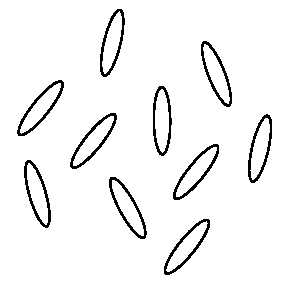
\includegraphics[width=0.8\textwidth]{../lessons/16_image/9.pdf}  \label{fig:16_9_1} }
\end{minipage}
\begin{minipage}[]{0.5\linewidth}
\centering
\subfloat[][Nematic phase]{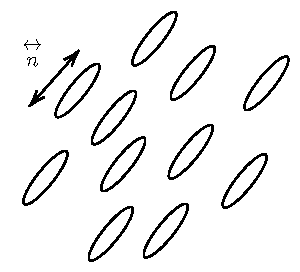
\includegraphics[width=0.8\textwidth]{../lessons/16_image/10.pdf}  \label{fig:16_9_2} }
\end{minipage}
\caption{\label{fig:} }
\end{figure}

\subsection{Order parameter}
A macroscopic definition of an order parameter for LC phase is based on the system response when subject to magnetic or electric fields. For instance, given an external magnetic field \( \va{H} \) the (diamagnetic) response of the system can be written as
\begin{equation}
  \va{M} = \bar{\bar{\chi } } \va{H}
\end{equation}
where the matrix \(  \bar{\bar{\chi } } \) is the response function.

In components
\begin{equation}
  M_ \alpha = \chi _{\alpha \beta } H _{\beta }
\end{equation}
with \( \alpha ,\beta =x,y,z \). For a static \( \va{H} \), \( \chi _{\alpha \beta } \) is symmetric.

 Clearly, for a isotropic fluid
\begin{equation}
  \chi _{\alpha \beta } = \chi  \delta _{\alpha \beta }
\end{equation}
For a LC in the neumatic phase one has
\begin{equation}
  \chi _{\alpha \beta } =
  \begin{pmatrix}
  \chi _\bot   &  0 & 0 \\
    0 &  \chi _ \bot & 0 \\
    0 &  0 &  \chi _\parallel
  \end{pmatrix}
\end{equation}
One can then define an order parameter based on \( \chi _{\alpha \beta } \) as
\begin{equation}
  Q_{\alpha \beta } = A \qty(\chi _{\alpha \beta } - \frac{1}{3} \delta _{\alpha \beta }\Tr \bar{\bar{\chi } }  )
\end{equation}
The order parameter is a second rank traceless tensor. It is possible to show that \(   Q_{\alpha \beta }  \) can be written in terms of the local average orientiational order of the elementary constituents, \(  \overset{\leftrightarrow}{n} (\va{r}) \) and the degree of local order given by a scalar \( S(\va{r}) \).
\begin{equation}
  Q_{\alpha \beta } (\va{r}) = S (\va{r}) \qty(n_{\alpha } (\va{r}) n_{\beta } (\va{r}) - \frac{1}{3}\delta _{\alpha \beta })
\end{equation}
Note that by construtction \( \bar{\bar{Q} }  \) is symmetric and traceless.

Its more general expression is
\begin{equation}
  Q_{\alpha \beta } =
  \begin{pmatrix}
  q_1   & q_2  & q_3 \\
  q_2   & q_4  & q_5 \\
  q_3   & q_5  & -q_1-q_4
  \end{pmatrix}
\end{equation}

\subsection{Landau free energy}
The free energy must be invariant to rotations of the system. Since \( Q_{\alpha \beta } \) transforms as a tensor under rotations, \( \mathcal{L} \) must be a combination of terms as \( \Tr \bar{\bar{Q} }^P \). By keeping terms up to fourth order
\begin{equation}
  \mathcal{L} = \mathcal{L}_0 + \frac{1}{2} A(T) \Tr \bar{\bar{Q} }^2 + \frac{1}{3} B(T) \Tr \bar{\bar{Q} }^3 + \frac{1}{4} C(T) \qty[ \qty(\Tr \bar{\bar{Q} }^2  )^2 + \Tr \bar{\bar{Q} }^4 ]
\end{equation}
In components,
\begin{equation}
  \mathcal{L} = \mathcal{L}_0 + \frac{1}{2} A(T) Q_{\alpha \beta }Q_{\beta \alpha } + \frac{1}{3} B(T) Q_{\alpha \beta } Q_{\beta \gamma  } Q_{\gamma  \alpha }+ \frac{1}{4} C(T) \qty(Q_{\alpha \beta } Q_{\beta  \alpha })^2
\end{equation}
\begin{remark}
Since each \( 3 \times 3 \) matrix satisfies the relation
\begin{equation}
   \Tr \bar{\bar{Q} }^4 = \frac{1}{2} \qty( \Tr \bar{\bar{Q} }^2)^2
\end{equation}
\end{remark}
the term proportional to \( C(T) \) can be written as \( \frac{1}{2}C(T)  \Tr \bar{\bar{Q} }^4 \).
\begin{remark}
The cubic term is here allowed since the rod like molecules have quadrupolar symmetry and the order parameter is a tensor for which the rotational invariance does not imply the absence of the odd powers.
\end{remark}
For the most general case of a \emph{biaxial nematic phase} \( \bar{\bar{Q} }  \) can be diagonalized giving
\begin{equation}
  Q_{\alpha \beta } =
  \begin{pmatrix}
  \frac{2}{3}s   & 0  & 0 \\
    0 &  - \frac{s+ \eta  }{3} & 0 \\
    0 &  0 & - \frac{(s- \eta  )}{3}
  \end{pmatrix}
\end{equation}
where \( \eta =0 \) corresponds to the standard uniaxial nematic phase.

In this cases
\begin{equation}
  Q_{\alpha \beta } =
  \begin{pmatrix}
  \frac{2}{3}s   & 0  & 0 \\
    0 &  - \frac{s  }{3} & 0 \\
    0 &  0 & - \frac{(s )}{3}
  \end{pmatrix}
\end{equation}
and
\begin{equation}
  \mathcal{L} = \mathcal{L}_0 + A(T) \frac{s^2}{3} + \frac{2}{27} B(T) s^3 + \frac{3}{81} C(T) s^4
\end{equation}
Assuming \( A(T) \simeq A (T-T^*) \), \( B(T) =B \) and \( C(T) = C \):
\begin{equation}
  \mathcal{L} = \mathcal{L}_0 + \frac{A}{3} (T-T^*) s^2 + \frac{2}{27} B s^3 + \frac{C}{9} s^4
\end{equation}
that has the same form of the one studied before for the first order phase transition.

In particular
\begin{equation}
  a = \frac{2}{3} A, \quad -w = \frac{2}{27} B, \quad b = \frac{2}{9} C
\end{equation}
It is then easy to see that the isotropic-nematic transition is of the first order and occur at
\begin{equation}
  T_t = \frac{w^2}{ba} + T^* = \frac{B^2}{27 A C} + T^*
\end{equation}











\section{Lesson}



As we approach the critical point \( T \rightarrow T_c \), the correlation length
\( \xi \sim \abs{T-T_c}^{-\nu }  \) diverges.

Maybe mean field is not a very good approximation in proximity of the critical point. Question: how bad is the mean field approximation in proximity of the critical point?
\begin{equation}
  \expval{S_i S_j} \overset{MF}{\rightarrow } \expval{S_i} \expval{S_j}
\end{equation}
Calculate the error:
\begin{equation}
  E_{ij} = \frac{ \abs{\expval{S_i S_j}  - \expval{S_i} \expval{S_j}}   }{\expval{S_i}\expval{S_j}  }
\end{equation}
Define
\begin{equation}
  G_c (i,j) \equiv \expval{S_i S_j} - \expval{S_i} \expval{S_j} = \expval{(S_i -\expval{S_i} )(S_j - \expval{S_j} )}
\end{equation}
If we want to compute the error in the mean field, is always zero. So, if we want calculate the average with respect to fluctuations it does not work. We can either look at the variation in which the field is the internal one, or we can somehow try to make a variation not because of thermal fluctuations but because we control it. We do this by using an external field. This is the response theory with a variation of the field.

In order to do that, instead using an \( H \) we use an \( H_i \).
\begin{equation}
  Z = \Tr_{\{ S \} } \qty(e^{-\beta \qty(-J \sum_{\expval{ij} }^{} S_i S_j   - \sum_{i}^{} H_i S_i ) } )
\end{equation}
The definition of the thermal average is
\begin{equation}
  \expval{S_i} = \frac{\Tr_{\{ S \} } \qty(S_i e^{-\beta \qty(-J \sum_{\expval{ij} }^{} S_i S_j   - \sum_{i}^{} H_i S_i ) } ) }{Z}
  = \beta ^{-1} \pdv{\ln{Z} }{H_i} = - \pdv{F}{H_i}
\end{equation}
\begin{equation}
  \expval{S_i S_j} = \frac{\beta ^{-1}}{Z} \frac{\partial^2{Z} }{\partial{H_i} \partial{H_j}  }
\end{equation}
\begin{equation}
  G_c (i,j) = \beta ^{-1} \frac{\partial^2{\ln{Z} } }{\partial{H_i} \partial{H_j}  }
  = - \frac{\partial^2{F(\{ H_i \}  )} }{\partial{H_i} \partial{H_j}  }
\end{equation}
\begin{equation}
  \pdv{}{H_j} \expval{S_i} = \pdv{}{H_j} \qty[-\pdv{F}{H_i} ] = G_c (i,j)
\end{equation}
\begin{equation}
  M = \sum_{i}^{} \expval{S_i}
\end{equation}
\begin{equation}
  \pdv{M}{H_j} = \sum_{i}^{} \pdv{\expval{S_i} }{H_j} = \sum_{i}^{} G_c (i,j)
\end{equation}
\begin{equation}
  H_j = H_j (H)
\end{equation}
\begin{equation}
  \pdv{M}{H} = \sum_{j}^{} \pdv{M}{H_j} \pdv{H_j}{H}
  =  \beta \sum_{ij}^{} G_c (i,j)
\end{equation}
the last one is the susceptibility \( \chi _T \).
 Therefore,
 \begin{equation}
   \chi _T = \beta \sum_{i,j}^{} G_c (i,j)
 \end{equation}
 \begin{equation}
   G_c (i,j) \rightarrow G_c (\abs{i-j} ) \sim G (\abs{\va{r}} )
 \end{equation}
More or less, we want to compute the total relative error
\begin{equation}
  E_{TT} = \frac{\int_{V_ \xi }^{ } \dd[D]{\va{r}}  G_c (r)}{ \int_{V_ \xi }^{} \dd[D]{\va{r}} \eta ^2 } \ll 1
\end{equation}
This quantity is related to \( \chi _T \). Because of the fluctutations we can say that the quantity above is
\begin{equation}
  \sim  \frac{\beta ^{-1} \chi _T }{ \int_{V_ \xi }^{} \dd[D]{\va{r}} \eta ^2 }
\end{equation}
where \( \chi _T \sim t^{-\gamma  } \) and  the denominator it is \(  \sim t^{2 \beta } \xi ^D\).
\begin{equation}
  \frac{t^{-\gamma  }}{t^{2 \beta } t^{-\nu D}}
\end{equation}
\begin{equation}
  E \overset{t \rightarrow 0}{\sim } ^{-\gamma -2 \beta + \nu D } \ll 1
\end{equation}
\begin{equation}
  - \gamma - 2 \beta + \nu D \ge 0 \Rightarrow D > \frac{\gamma + 2 \beta  }{\nu }
\end{equation}
this is called the \emph{Ginzburg criterium}.

In the mean field we have: \( \gamma =1  \), \( \beta = 1/2 \). We obtain:
\begin{equation}
  D > \frac{2}{\nu }
\end{equation}
We have \( \nu _{MF} = 1/2 \). THerefore the dimension is \( D>4 \) for the mean field.
The
\begin{equation}
  D_c = \frac{\gamma + 2 \beta  }{2}
\end{equation}
is called \emph{upper critical dimension}.

Now we have a lower critical dimension (remember the last lessons!!) and an upper one.







\end{document}
